%!TEX root=../thesis.tex
\chapter{The PROSIT tool}\label{chp:tool}

% + LA BASE DA CUI PARTIRE E' IL PAPER \ref{prosit}
% + struttura dei moduli principali + linguaggio + librerie utilizzate + OOP patterns 
% + use cases diagram (vedi paper) 
% + focus nella creazione dei task RR (qbd_rr_colver.cpp) e di come abbiamo migliorato
%   la creazione della matrice (costruita in 3 fasi separate) in modo da sfruttare a pieno
%   le regolarità presenti al suo interno --> dati su quanto siano migliorate le performance 
%   dopo le modifiche (vedi mail con Bernardo per i numeri)
% + approssimazione conservativa della PMF (sia in alto che in basso)
% - distinzione solver da linea di comando e per xml
%     [-] solver_command_line e descrizione parametri in input
%     [-] xml_solver con esempi di chiamata + spiegazione struttura dell'xml da dare in input
% - descrizione web interface e motivi per cui è stata fatta (facilità d'uso per la creazione
%   dell'xml da zero)

\section{Internal structure}
PROSIT is written in C++ and has a modular structure, as Object Oriented Programming (OOP) implicitly suggests to use.\\
Some external libraries have been used in order to increase the performance during the matrices/vectors operarions and to simplify some others. The most important ones are \emph{Eigen}\footnote{\url{http://eigen.tuxfamily.org}}, \emph{TinyXML-2}\footnote{\url{https://github.com/leethomason/tinyxml2}} and \emph{Doxygen}\footnote{\url{http://www.stack.nl/~dimitri/doxygen/}}.\\   
Eigen is the most important library for the tool's core: it is versatile, because it supports matrices and vectors of all sizes (both fixed and dynamic) with a lot of primarys operarions already implemented, it is reliable and very fast, because performance can become a real problem when the matrices have several hundreds of rows and columns.\\
The second one is TinyXML-2, which has been used in the parser for the XML files that are used as solver's inputs. It provides APIs to accesso to the XML inner structure (which is treated as a Document Object Model) as a C++ object that can be easily browsed and manipulated.\\
The latter is Doxygen, a documentation generator for multiple programming languages. It is widely used in projects\footnote{A list of some projects which already use this tool to generate their documentation is available at \url{http://www.stack.nl/~dimitri/doxygen/projects.html}} because it is highly configurable, it can extract code structure (like class diagrams and many others) even from undocumented files and especially because it is possible to select the output format for the documentation (such as HTML, {\LaTeX} and Unix man pages).\\
The tool can be devided into some standalone modules:
\begin{itemize}
  \item the distribution handler class, for both PMFs and CDFs.
  \item the task descriptor class, where the inner structure of a task is described and stored.
  \item the XML parser and the utilities for the XML manipulation.
  \item the probability solver class, which is essentialy a wrapper object for the solving algorithm and the parameters for the RR task.
  \item the QBDP interpretation for the input task; it is the class that actually implements the functions to build the transition matrix and the solution algorithm for the probability solver class.
  \item the QoS function, which is used to compute the final value for the quality of service, given the input task parameters.
  \item the command line and the XML solvers are those which contains the main function that are compiled in order to obtain the executable files.
\end{itemize}

\begin{figure}[H]
  \center{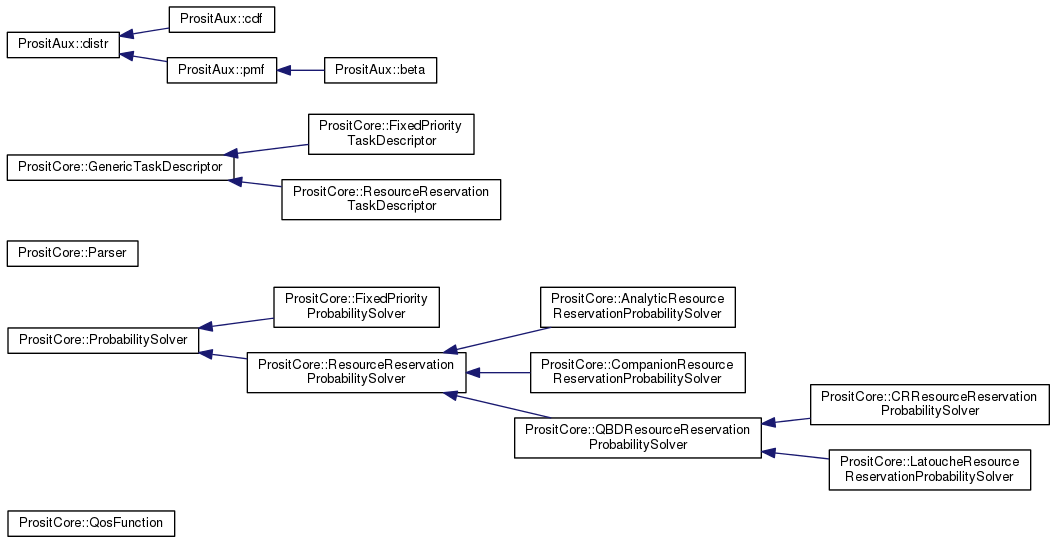
\includegraphics[width=0.9\linewidth]{classdiagram.png}}
  \caption{The class diagram generated by Doxygen.}
  \label{automaton}
\end{figure}

\section{Use cases}
The most common use case for PROSIT is the \emph{analysis problem}: the designer is required to enter the parameters to define the task he/she wishes to analyse.\\
Since a task can only be of  the resource reservation type\footnote{The fixed priority type of task is currently under development and it is not available yet.}, the values for the time requirements (the PMF for the computation time and the one for the interarrival time, which is essential if the task is aperiodic) and the scheduling parameters \( Q_{i}^s \) and \( T_{i}^s \) must be provided. Thanks to the temporal isolation property defined in Equation \ref{schedCond}, if several tasks are passed as inputs, the tool is allowed to treat every task on its own. It is possible to easily understand that this situation leads to additional semplifications during the design phase.\\ 
The probability distribution functions can be specified either inside the task definition or taken as input from a file.
\begin{figure}[H]
  \center{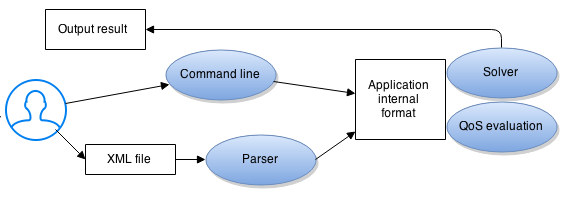
\includegraphics[width=0.7\linewidth]{usecase.png}}
  \caption{The analysis use case.}
  \label{usecase}
\end{figure}

As a result of a tool invocation, all the provided information are analysed and then the solver for the probabilistic deadlines is called. The \emph{apply\_algorithm()} method called by the probability solver object is a pure virtual function\footnote{Pure virtual functions in C++ are used to take advantage of polymorphism. This is essential for providing a unique interface for multiple objects which implements different versions of the same method, based on the input values.}; this allows PROSIT to call the right solution strategy selected by the user.\\
The final results and their computation times are printed either on the screen or dumped on a text file.

\section{RR solver}
The solver for resource reservation tasks is based on algorithms for a numerical solution of the connected quasi-birth death process and implements the following methods:
\begin{lstlisting}[frame=bt]
  void pre_process();
  bool compute_pi0();
  void post_process();
  void fill_in_probability_map();
\end{lstlisting}
The \emph{pre\_process()} function creates the matrices used by the QBD algorithms, which are implemented in every sublclass under the name of \emph{apply\_algorithm()}. The second method is responsible of computing the probabilities from the matrix computed in the previous step. At the end \emph{post\_process()} guarantees that the algorithm gives a reasonable output, while the last method fills the map which is used to store te computation results.\\
The functions described above are invoked by the solver in the order in which they were presented.

\subsection{Conservative approximation for PMF}
Before building the transition matrix, the values of the PMFs for both computation and interarrival times need a \emph{resampling} to an integer value\footnote{In the probabilistic deadline \emph{(t,p)}, both values can be expressed as floating point numbers; then, internally, PROSIT approximate them to an integer since we aim to output an estimate.}, in order to obtain a \emph{conservative approximation}.\\
The way of reasoning is the same for both cases, but with a very important detail: a computation time has to be approximated to a greater value, while an interarrival time to a lower one.\\ 
This has to be done in this way because the tool must always be placed into a \emph{worst-case scenario}. The resampling function returns a pointer to the resampled PMF object and it is defined as follows:
\begin{lstlisting}[frame=bt]
  pmf * resample(int granularity, bool direction);
\end{lstlisting}

where \emph{granularity} is the desired number of bins for the resampled PMF and \emph{direction} is a flag which is used to make an approximation either to a grater or a lower value.\\
\begin{figure}[H]
  \center{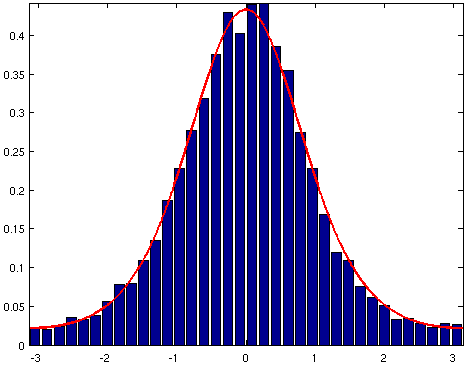
\includegraphics[width=0.4\linewidth]{resample.png}}
  \caption{A normal distribution (in red) resampled at 36 bins (in blue).}
  \label{resample}
\end{figure}

\subsection{Transition matrix creation}
The creation of the transition matrix which is later used to apply the algorithms can result in a critical performance bottleneck, since the size can be huge\footnote{Some tests we performed developing the tool run the algorithms on a matrix with a size of nearly one thousand.}. Given that the complexity of the algorithms mentioned in Section \ref{benefits} cannot be changed, this will certainly explain the motivation behind the effort to optimize as much as possible the matrix creation phase.\\
As explained in \ref{transitionmatrix}, the whole transition matrix has a recurrent block structure.\\ 
The first step is to limit the matrix size to the one of \( C \), \( A_{0} \), \( A_{1} \) and \( A_{2} \), since it can be theoretically have an infinite size that makes it intractable computationally speaking. Firstly the values for \( max_{rows} \) and \( max_{cols} \) need to be computed, which represent the maximum possible number of rows and columns respectively.\\ 
They can be evaluated as follows: 
\begin{equation*}
\begin{split}
  max_{rows} &= i.get_min() * Q + 1 \\
  max_{cols} &= c.get_max() + 1
\end{split}
\end{equation*}

where \( i.get\_min() \) returns the minimum value for the interarrival time PMF, \( c.get\_max() \) returns the maximum value for the computation time PMF and \( Q \) is the budget associated with the given task.\\
Then, after taking \( max_{v} = max\{max_{rows}\,,\,max_{cols}\} \) as the size of one of the above mentioned matrices, it is possible to know that the size of the whole transition matrix is \( 2 \times max_{v} \).\\
The approach used to calculate the values inside the matrix is based on its internal structure, which is in proven\cite{pipelines} to be like:
\begin{figure}[H] \label{matrixstructure}
\begin{equation*} 
  P_{i} = 
  \begin{bmatrix}
    a_{i,0} & a_{i,1} & a_{i,H_{i}} & 0 & 0 & 0 & 0 & 0 & 0 & 0 \\
    \vdots & \vdots & \vdots & \vdots & \vdots & \vdots & \vdots & \vdots & \vdots & \vdots\\
    a_{i,0} & a_{i,1} & a_{i,H_{i}} & 0 & \cdots & \cdots & \cdots & \cdots & \cdots & \cdots \\
    b_{i,0,0} & b_{i,0,1} & b_{i,0,H_{i}} & b_{i,0,H_{i}+1} & 0 & \cdots & \cdots & \cdots & \cdots & \cdots \\
    b_{i,0,0} & b_{i,0,1} & b_{i,0,H_{i}} & b_{i,0,H_{i}+1} & b_{i,0,H_{i}+2} & 0 & \cdots & \cdots & \cdots \\
    \vdots & \vdots & \vdots & \vdots & \vdots & \vdots & \ddots & \vdots & \vdots & \vdots \\
    b_{i,G_{i},0} & b_{i,G_{i},1} & \cdots & b_{i,G_{i},H_{i}} & b_{i,G_{i},H_{i}+1} & \cdots & \cdots & b_{i,G_{i},F_{i}} & 0 & \cdots \\
    0 & c_{i,0} & c_{i,1} & \cdots & c_{i,H_{i}} & c_{i,H_{i}+1} & \cdots & c_{i,F_{i}-1} & c_{i,F_{i}} & \ddots \\
    \vdots & \ddots & \ddots & \ddots & \ddots & \ddots & \ddots & \ddots & \ddots & \ddots
  \end{bmatrix}
\end{equation*}
\caption{The transition matrix for the generic \( i^{th} \) stage.}
\end{figure}

In the \( P_{i} \) matrix described in Figure shonw above it is possible to spot an internal recurrent configuration, which is highlighted with the different names for the rows \emph{a}, \emph{b} and \emph{c}.\\
To take advantage of this proprerty, the \emph{pre\_process()} method builds the matrix in three steps: the first one is to calculate only the first \emph{a}-row block and then copy its value until the end of it. Secondly all the \emph{transient}\footnote{This part of the matrix exists only if the task is aperiodic. In the case of a periodic one, this part of the matrix does not exists and the transition matrix is composed only by the blocks named with \emph{a} and \emph{c}.} rows denoted with the letter \emph{b} are calculated, cell by cell. In the \emph{c} block, as happened for the first one, only the first row is calculated and then it is copied to the following one shifted right by one.\\
Instead of calculating every single cell of the matrix, which needs a function to be called \( max_{v}^{2} \) times, opting for a solution like this one was not an option. The time needed to calculate the entire matrix with the new method decreased of around 40\%, even though the overall complexity is still an \( O(n^{2}) \). For more details about the results, see Chapter \ref{????????}.
%
% TODO: reference to the results of the gain in speed of the method
%       see Bernardo's email with the values
% 
